For the next part of the report we are going to be visualizing the testing process as well as 
using images from outside the dataset to see how well our model preforms in a real world scenario.
The script has 3 modes:
\begin{itemize}
    \item \textbf{Random CIFAR-10 image:} Get a random image from the CIFAR-10 test batch and evaluate 
    it in real-time.
    \item \textbf{Custom image:} Provide a random image from storage to evaluate in real-time.
    \item \textbf{Manual batch:} Iterate throughout all the images inside the \textit{manual-batch/} folder 
    and return the approximate real world accuracy of the model.
\end{itemize}

The first two modes show the image being tested and the predicted class. The first also shows the 
true class which is embedded into the dataset. FInally the third mode compares automatically the 
predicted class with the true class, which can be found in the image's filename. Let's have a look
at the different out puts:
\begin{itemize}
    \item \textbf{Random CIFAR-10 image:} 
    \begin{figure}[H]
        \centering
        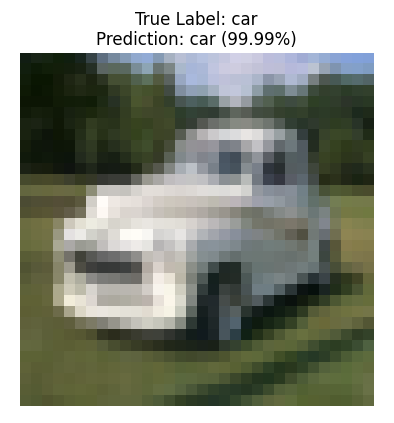
\includegraphics[width=0.5\textwidth]{media/random_cifar.png}
        \caption{Random CIFAR-10 image}
    \end{figure}
    \item \textbf{Custom image:} 
    \begin{figure}[H]
        \centering
        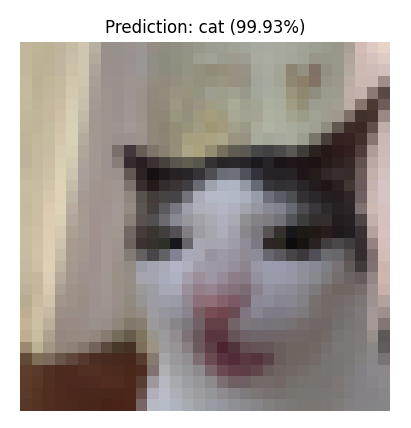
\includegraphics[width=0.5\textwidth]{media/custom_image.png}
        \caption{Custom image}
    \end{figure}
    \item \textbf{Manual batch:} 
    \begin{figure}[H]
        \centering
        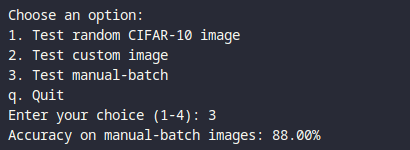
\includegraphics[width=0.5\textwidth]{media/manual_batch.png}
        \caption{Manual batch}
    \end{figure}
\end{itemize}

Luckily, the real world accuracy proved to be not too far off the testing accuracy. Truth be told,
the custom images were not very challenging. The objects were centered, in good lighting and taken
from a good angle. Nonetheless, the model was able to perform well on unknown data.